
\section{Aprendizaje}\label{aprendizaje}
En aprendizaje de m\'aquinas el aprendizaje por refuerzamiento es una forma de plantear el problema de inteligencia completamente distinta a el aprendizaje supervisado o no supervisado que generalmente está basado en ejemplos y un par entrada/salida, el objetivo del agente es aprender la funci\'on que haya producido esos pares. Sim embargo no siempre existe un supervisor que pueda verificar los resultados otorgados.
Existen ambientes en la vida real donde al agente no se le proporciona ni el supervisor ni los ejemplos, en donde se comienza sin contar con un modelo del ambiente o una funci\'on de utilidad. En estos casos la aplicaci\'on del aprendizaje por reforzamiento es la más indicada \cite{peterAndNorvig}.

La t\'ecnica de refuerzo es aplicada en la vida diaria constantemente, pues está basada en comportamientos. Es la forma en que se entrena a una mascota, es la manera en que un bebé logra aprender a sujetar objetos, esos son ejemplos de los muchos en los que en la realidad aparece esta t\'ecnica de aprendizaje.

Cuando es aplicada a inteligencia artificial las bases son las mismas, obviamente a un robot no se le podr\'a dar una galleta literalmente como premio de su buena acci\'on o quitarle la televisi\'on como castigo.
 
Existen varias estrategias que permiten otorgar recompensas positivas o negativas a un agente, en este caso un robot, con ellas ir moldealdo el comportamiento que se considere correcto.

Un algoritmo para aprender por reforzamiento es aprendizaje-Q, que es el utilizado para que Junny aprenda a acercarse a la pelota.
 
%En el área de inteligencia artificial, asociada a robótica, existen variadas técnicas que permiten que un robot pueda aprender a realizar alguna tarea. En este caso particular se utiliz\'o la técnica de aprendizaje por reforzamiento que consiste en dar recompensas positivas o negativas dependiendo del desempeño del robot.


Según \cite{Mitchell} todo aprendizaje se define por la realización de una tarea $T$, cuyo desempeño medido por $D$, mejora con la experiencia $E$. En la investigación presente la tarea $T$ es aprender cuál es el mejor conjunto de ``acciones de movimiento" que se debe tomar con la finalidad de acercarse a la pelota. La experiencia $E$ se da a través un conjunto de pruebas, en las que Junny debe buscar la pelota y posicionarse frente a ella. El desempeño $D$ se mide con respecto a si el robot logra posicionar la pelota en el área de pateo y cuántas acciones de movimiento son necesarias para lograrlo.

Como existe incertidumbre con respecto a la dinámica del ambiente (esto es, no se conoce la función $\delta(s,a)$, definida en la subsección \ref{subsec:Qlearning} se utilizó el modelo de aprendizaje Q-learning, el cual permite mejorar el desempeño de la tarea definida en base a la experiencia de cada prueba. A continuación se presenta y describe la configuración de las caracter\'isticas particulares del aprendizaje utilizado para este proyecto.

\subsection{Modelo del problema}

El algoritmo para Q-learning se adapta a problemas configurados como procesos de decisión Markovianos (MDP). En este tipo de problemas el resultado de aplicar una acción en un estado particular depende solo de ese estado y esa acción, no de las acciones del pasado. 

En un MDP, un agente representa su mundo a través de un conjunto de estados y tiene un conjunto de acciones que puede ejecutar. Cada vez que el agente identifica el estado en el que se encuentra y escoge una acción para tomar, dependiendo del resultado, este recibe una recompensa determinada.

En la sección \ref{estados} se define el conjunto de estados que conforman el mundo de Junny. En la secci\'on \ref{sec:acciones} se dan a conocer las posibles acciones definidas y en la secci\'on \ref{recompensas} se define la ecuaci\'on para calcular las recompensas.   

\subsubsection{Estados}\label{estados}

De forma general se puede decir que los estados se encuentran definidos en función de la posición de la pelota con respecto al robot. En la sección \ref{mundo} se ha explicado la manera en la que se representa el mundo en base a 13 regiones en las que se puede encontrar la pelota. Para el aprendizaje se ha decidido ampliar el número de regiones para afinar y mejorar el tiempo en el que se llega a la pelota. Estas regiones se muestran el la figura ~\ref{fig:estados2}.

Cada región en la que se pueda detectar la pelota es un estado diferente. Por lo tanto se generan 18 estados, 17 de ellos se corresponden con la detección de la pelota en cada una de las regiones que se muestran en la imagen ~\ref{fig:estados2} y el estado número 18 representa la ocasión en la que no se logra ubicar la pelota en ninguna de las regiones.  

\begin{figure}[hbtp]
\centering
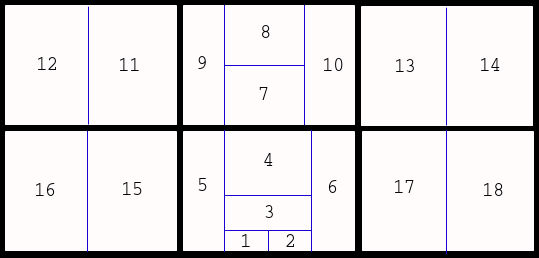
\includegraphics[scale=0.5]{imagenes/Regiones2.jpg}
\caption{Estados definidos seg\'un la región en la que se detecta la pelota}
\label{fig:estados2}
\end{figure}


\subsubsection{Acciones}\label{sec:acciones}

Las posibles acciones a realizar son un subconjunto de las acciones de movimiento definidas en la sección \ref{esqueleto}. Además se agregaron otras acciones para mejorar el desempeño en la búsqueda de la pelota. Las acciones disponibles son:

\begin{itemize}
\item {Caminar un paso hacia adelante (2.5 cm)}
\item {Caminar dos pasos hacia adelante (4.8 cm)}
\item {Caminar cuatro pasos hacia adelante (9.9 cm)}
\item {Girar a la izquierda (3 cm)}
\item {Girar doble a la izquierda (6 cm)} 
\item {Girar a la derecha (3 cm) }
\item {Girar doble a la derecha (6 cm)}
\label{item:todaslasacciones}
\end{itemize}

\subsubsection{Recompensas}\label{recompensas}

La recompensa, que puede ser positiva o negativa, se otorga a un par $(s,a)$, en donde $s$ es un estado y $a$ es una acci\'on. Se calcula en base a que tanto el robot se acerca a la pelota cuando en el estado $s$ se toma la acci\'on $a$. Es decir, las recompensas se definen en base a la distancia recorrida, con respecto a la pelota, cuando se toma una acci\'on.  

La distancia de una región con respecto al área de pateo, se define con la función $d: r \rightarrow y$ con $r \in \{1,2,3 ...18\}$ y $y \in \{1,2,3 ...10\}$. En donde $r$ es el número de la región y $y$ es la distancia de la región con respecto al \'area de pateo. Se asign\'o una distancia a cada regi\'on como se muestra en la figura ~\ref{fig:distancias}. El valor 1 se le asigna a las regiones m\'as cercanas al robot (zonas de pateo), $d(1)= 1$ y $d(2)=1$; el valor 10, a las regiones m\'as lejanas (regiones 12 y 14). Adicionalmente se define la distancia de la región 18 como $d(18)=10$. 
     
\begin{figure}[hbtp]
\centering
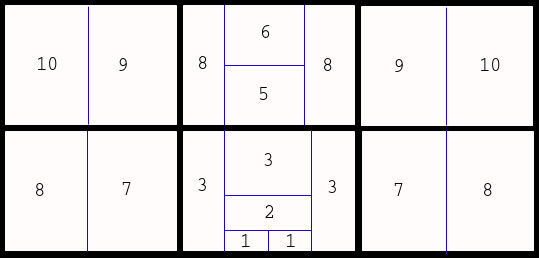
\includegraphics[scale=0.5]{imagenes/Distancias2.jpg}
\caption{Distancias relativas de la pelota establecidas para otorgar la recompensa.}
\label{fig:distancias}
\end{figure}

Junny gana una recompensa positiva cuando, con una acción, la pelota pasa de una región de mayor valor (lejana) a una de menor valor (más cercana). Si la pelota se mantiene en la misma región obtiene recompensa 0. De lo contrario obtiene una recompensa negativa. La ecuación se define como:



\begin{equation}
R(s,a,s') = \dfrac{d(s) - d(s')}{10}
\end{equation}


El rango de valores para la recompensa se encuentra entre -1 y 1. 


\subsection{Elecci\'on de la acci\'on}\label{subsec:eleccionAccion}

Se entiende que dado un estado $s$ se tienen 7 posibles acciones $\{a_1, a_2, ... a_7\}$ que, en el entrenamiento del robot, él aprende cuál es la mejor a realizar según el estado en el que se encuentra. A mayor valor de $Q(s,a)$ mejor es la acción $a$. Si siempre se toma el máximo valor se favorece la explotación. Si se toman acciones aleatorias se favorece la exploración. Para que el aprendizaje obtenga buenos resultados se debe tener un equilibrio entre la exploración y la explotación. 

Para variar entre la explotación y la exploración se utiliz\'o la función de probabilidad definida como  %\[P(a_{i} | s) = \dfrac{k^{Q(s,a_{i})}}{\sum_{j}k^{Q(s,a_{j})}}  \] 


\begin{equation}
 P(a_{i} | s) = \dfrac{k^{Q(s,a_{i})}}{\sum_{j}k^{Q(s,a_{j})}}
\end{equation}

Con valores diferentes de $k$ para cada conjunto de pruebas, como se explica en el capítulo \ref{chapter:resultados}.  
 
 
\subsection{Actualizaci\'on de Q(s,a)}

La actualizaci\'on de Q(s,a) se define por la siguiente formula 
 
\begin{equation}
Q (s,a) = r + {\gamma\max_{a'}} Q(\delta(s ,a ) , a') 
\end{equation} 



Donde $r$ y $\max_{a'} Q(\delta(s,a),a')$ se explican en la subsecci\'on \ref{subsec:Qlearning} el factor $\gamma$ es el factor de descuento que varia de \[   0 \leq  \gamma < 1 \] este par\'ametro es arbitrario y se debe ajustar durante el aprendizaje, en el cap\'itulo \ref{chapter:resultados}  se presentan los $\gamma$ utilizados para los entrenamientos.